\documentclass[a4paper, 14pt]{extreport}
\usepackage[utf8]{inputenc}
\usepackage[english,russian]{babel}
\usepackage{amssymb,amsfonts,amsmath,mathtext,cite,enumerate,float}
\usepackage{pgfplots}
\usepackage{graphicx}
\usepackage[inkscapeformat=png]{svg}
\usepackage{tocloft}
\usepackage{listings}
\usepackage{caption}
\usepackage{tempora}
\usepackage{titlesec}
\usepackage{setspace}
\usepackage{geometry}
\usepackage{indentfirst}
\usepackage{pdfpages}
\usepackage{enumerate,letltxmacro}
\usepackage{threeparttable}
\usepackage{hyperref}
\usepackage{flafter}
\usepackage{enumitem}
\usepackage{multirow}
\usepackage{mathtools}
\usepackage{longtable}
\usepackage[figure,table]{totalcount}
\usepackage{lastpage}

\lstdefinestyle{code}{
	basicstyle=\footnotesize\ttfamily,
	frame=single,
	tabsize=4,	
	breaklines=true
}

\setlist{nosep}
\hypersetup{pdfborder=0 0 0}

\newcommand{\ssr}[1]{\begin{center}
		\LARGE\bfseries{#1}
	\end{center} \addcontentsline{toc}{chapter}{#1}  }

\makeatletter
\renewcommand\LARGE{\@setfontsize\LARGE{22pt}{20}}
\renewcommand\Large{\@setfontsize\Large{20pt}{20}}
\renewcommand\large{\@setfontsize\large{16pt}{20}}
\makeatother

\RequirePackage{titlesec}
\titleformat{\chapter}[block]{\hspace{\parindent}\large\bfseries}{\thechapter}{0.5em}{\large\bfseries\raggedright}
\titleformat{name=\chapter,numberless}[block]{\hspace{\parindent}}{}{0pt}{\large\bfseries\centering}
\titleformat{\section}[block]{\hspace{\parindent}\large\bfseries}{\thesection}{0.5em}{\large\bfseries\raggedright}
\titleformat{\subsection}[block]{\hspace{\parindent}\large\bfseries}{\thesubsection}{0.5em}{\large\bfseries\raggedright}
\titleformat{\subsubsection}[block]{\hspace{\parindent}\large\bfseries}{\thesubsection}{0.5em}{\large\bfseries\raggedright}
\titlespacing{\chapter}{12.5mm}{-22pt}{10pt}
\titlespacing{\section}{12.5mm}{10pt}{10pt}
\titlespacing{\subsection}{12.5mm}{10pt}{10pt}
\titlespacing{\subsubsection}{12.5mm}{10pt}{10pt}

\makeatletter
\renewcommand{\@biblabel}[1]{#1.}
\makeatother

\geometry{left=30mm}
\geometry{right=10mm}
\geometry{top=20mm}
\geometry{bottom=20mm}

\onehalfspacing

\renewcommand{\vec}[1]{\overrightarrow{#1}}
\renewcommand{\theenumi}{\arabic{enumi}}
\renewcommand{\labelenumi}{\arabic{enumi}\text{)}}
\renewcommand{\theenumii}{.\arabic{enumii}}
\renewcommand{\labelenumii}{\asbuk{enumii}\text{)}}
\renewcommand{\theenumiii}{.\arabic{enumiii}}
\renewcommand{\labelenumiii}{\arabic{enumi}.\arabic{enumii}.\arabic{enumiii}.}

\renewcommand{\cftchapleader}{\cftdotfill{\cftdotsep}}

\addto\captionsrussian{\renewcommand{\figurename}{Рисунок}}
\DeclareCaptionLabelSeparator{dash}{~---~}
\captionsetup{labelsep=dash}

\captionsetup[figure]{justification=centering,labelsep=dash}
\captionsetup[table]{labelsep=dash,justification=raggedright,singlelinecheck=off}
\captionsetup[lstlisting]{labelsep=dash,justification=raggedright,singlelinecheck=off}

\newcommand{\floor}[1]{\lfloor #1 \rfloor}

\pgfplotsset{width=0.85\linewidth, height=0.5\columnwidth}

\linespread{1.3}

\parindent=1.25cm

\def\labelitemi{---}
\setlist[itemize]{leftmargin=1.25cm, itemindent=0.65cm}
\setlist[enumerate]{leftmargin=1.25cm, itemindent=0.55cm}

\newcommand{\specialcell}[2][c]{%
	\begin{tabular}[#1]{@{}c@{}}#2\end{tabular}}
\frenchspacing



\begin{document}
\setcounter{page}{3}
\ssr{РЕФЕРАТ}

Расчетно-пояснительная записка 15 c., 2 рис., 11 ист., 2 табл., 1 прил.

Ключевые слова: методы хранения временных рядов, методжы прогнозирования временных рядов, методы оптимизации, 
модели машинного обучения, случайный лес, регрессия, решающие деревья, гауссовский процесс.

Объект исследования: методы хранения и прогнозирования временных рядов.

Цель работы: исследование методов хранения и прогнозирование временных рядов.

В работе выполняется формализация задачи прогнозирования временных рядов, рассмотрение методов решения задачи
и сравнение методов.

\clearpage\setlength{\cftbeforetoctitleskip}{-4mm}
\renewcommand{\contentsname}{\makebox[\textwidth][c]{\LargeСОДЕРЖАНИЕ}}
\tableofcontents

\clearpage\ssr{ВВЕДЕНИЕ}

Авторегрессионные модели (AR) являются фундаментальной концепцией в анализе и прогнозировании временных рядов. Их 
часто применяют в различных областях, включая финансы, экономику, климатологию и многое другое.

Научные работы о прогнозировании временных рядов появились еще в 1970 году в труде Бокса~\cite{box}. Бокс рассматривает 
линейные стационарные модели и некоторые системы, сводящиеся к ним. В частности, рассматривается модель ARIMA и ее 
производные, учитывающие сезонность и внешние факторы.

Значительный вклад в развитие прогнозирования временных рядов внесла работа о LSTM~\cite{martin} в 2012 году, в которой 
рассматривалась модификация рекурентной нейронной сети для задач распознавания речи. Появляется множество статей, в 
которых модель LSTM с некоторыми модификациями превосходит в точности все ранее известные модели~\cite{china}.

В это же время исследуется вопрос построения ансамблей моделей, когда на основе множества «простых» моделей обучается 
другой алгоритм регрессии, минимизирующий общую ошибку. 

Целью данной работы является исследование методов хранения и прогнозирования временных рядов.

Для достижения поставленной цели необходимо выполнить следующие задачи:
\begin{itemize}
	\item[---] формализовать задачу прогнозирования временных рядов;
	\item[---] проанализировать основные известные методы решения;
	\item[---] сравнить методы решения по заранее сформулированным критериям.
\end{itemize}

\chapter{Формализация задачи}

Схема формализации задачи в виде диаграммы IDEF0 представлена на рисунке~\ref{idef}.

\begin{figure}[h]
	\centering
	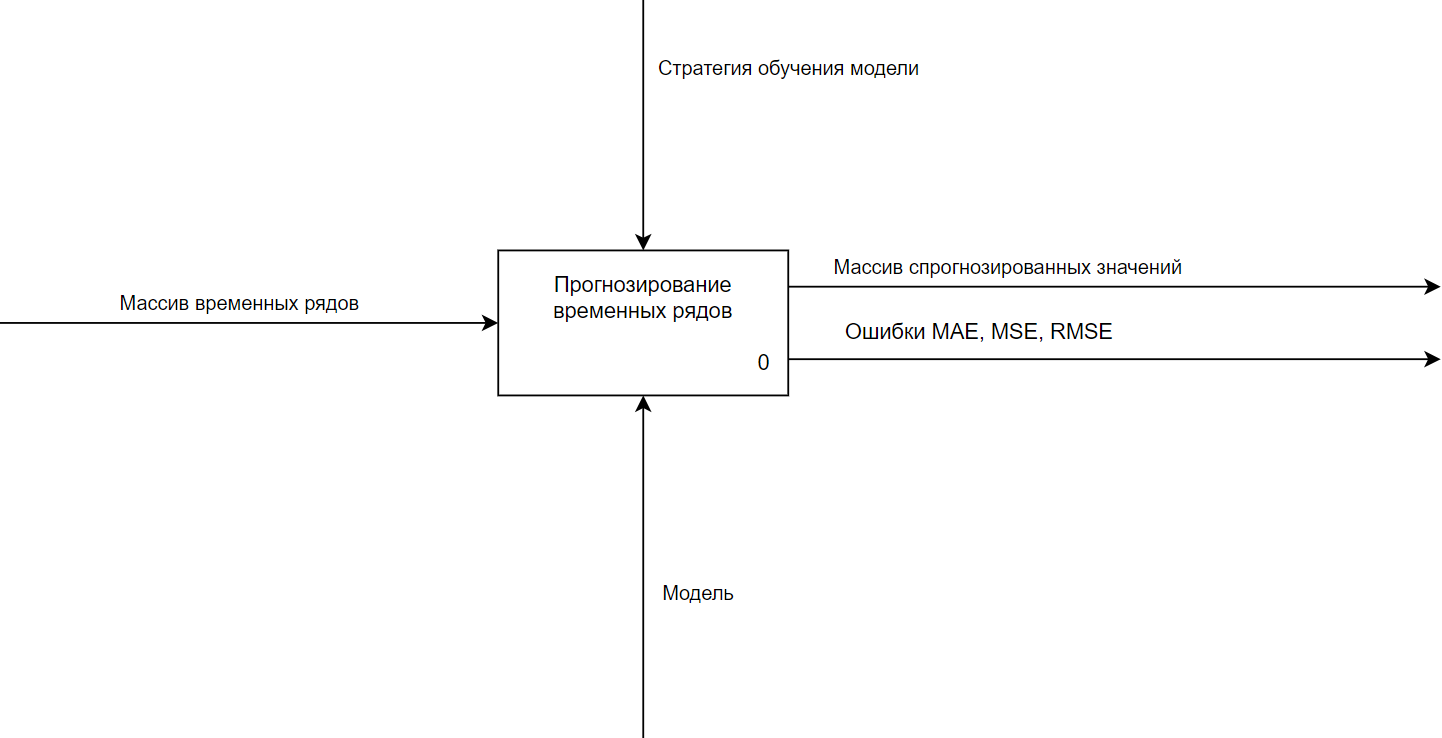
\includegraphics[scale=0.55]{tools/idef.png}
	\caption{IDEF0 диаграмма}
	\label{idef}
\end{figure}

\section{Математическая формулировка}

Даны временные ряды 
\begin{equation}
	X_{i} =\{x_{i,t}, t = \overline{1,k}\}, i = \overline{1, m}
\end{equation}
где $m$~--- количество временных рядов, а $k$~--- размер временного ряда~\cite{mayorova}.

Задача состоит в том, чтобы построить такую модель $A(X_{i})$, что
\begin{equation}
	 A(X_{i}) = x_{i,k+n}
\end{equation}
где $n$ количество значений, которые необходимо спрогнозировать~\cite{mayorova}.

При этом дополнительным условием является минимизация одной из ошибок MAE (Mean Abcolute Error), представленную 
формулой~\ref{MAE} или MSE (Mean Square Error), представленную формулой~\ref{MSE} для каждого временного ряда.
\begin{equation}
	\label{MAE}
	 MAE = \sum \limits _{i=k+1}^{k+n} \frac{|y_{i}-x_{i}|}{n}
\end{equation}

\begin{equation}
	\label{MSE}
	 MSE = \sum \limits _{i=k+1}^{k+n} \frac{(y_{i}-x_{i})^2}{n}
\end{equation}

В этих формулах $y_{i}$ --- истинное значение временного ряда, а $x_{i}$ --- спрогнозированное~\cite{itmo}.

\chapter{Анализ методов прогнозирования временных рядов}

Временной ряд --- это ряд точек данных, индексированных во временном порядке~\cite{deeplearning}. Чаще всего временной 
ряд --- это последовательность, взятая в упорядоченных равноотстоящих точках времени. Таким образом, это
последовательность дискретных временных данных.

Значения временного ряда является суммой его четырех основных компонент~\cite{kizbek}:
\begin{itemize}
	\item[---] тренд --- плавно меняющаяся компонента, описывающая чистое влияние долговременных факторов, т. е. 
	длительную тенденцию изменения признака (например, рост населения);
	\item[---] сезонность --- компонента, отражающая повторяемость экономических процессов в течение не очень 
	длительного периода (например, объем продаж товаров или перевозок пассажиров в различные времена года);
	\item[---] цикличность --- компонента, отражающая повторяемость экономических процессов в течение длительных 
	периодов (например, влияние волн экономической активности Кондратьева);
	\item[---] шум --- случайная компонента, отражающая влияние не поддающихся учету и регистрации случайных факторов.
\end{itemize}

Чаще всего временные ряды хранят в виде массива значений, индексированного по времени, но иногда предпочитают хранить 
отдельно все компоненты ряда.

В этом разделе рассматриваются некоторые методы прогнозирования временных рядов. 

\section{ARIMA}

ARIMA (Autoregressive Integrated Moving Average) --- это модель авторегрессии с интегрированной скользящей средней. 
Определяется тремя параметрами: (p, d, q).
\begin{itemize}
	\item[---] авторегрессия AR( p ) --- регрессионная модель, которая использует зависимую связь между текущим 
	наблюдением наблюдениями за предыдущий период;
	\item[---] интеграция I( d )  --- использует дифференциацию наблюдений, чтобы сделать временной ряд стационарным. 
	Дифференциация включает вычитание текущих значений ряда из его предыдущих значений d раз;
	\item[---] скользящее среднее MA( q ) --- модель, которая использует зависимость между наблюдением и остаточной 
	ошибкой из модели скользящего среднего, применяемой к запаздывающим наблюдениям. Порядок q представляет собой 
	количество членов, которые должны быть включены в модель.
\end{itemize}

Значения временного ряда считаются по следующей формуле~\ref{ARIMA}.
\begin{equation}
	\label{ARIMA}
	 X_i = c + \varepsilon_i +\sum \limits _{k=1}^{p} \alpha_kX_{i-k} +\sum \limits _{k=1}^{q} \beta_k\varepsilon_{i-k}
\end{equation}
где $c$ --- некоторая константа, $\varepsilon_{i}$ --- значение шума, $\alpha_{k}$ --- коэффициенты авторегрессии, $\beta_{k}$ ---
коэффициенты скользящего среднего~\cite{kizbek}.

Недостатком этой модели является то, что она плохо справляется с данными, в которых ярко выражена компонента 
сезонности~\cite{kizbek}.

\section{SARIMA}

SARIMA (Seasonal Autoregressive Integrated Moving Average) --- это расширение несезонной модели ARIMA, разработанное для 
обработки данных с сезонными закономерностями. Определяется четырьмя параметрами: (p, d, q, s).

Параметры (p, d, q) аналогичны параметрам модели ARIMA. Параметр s представляет сезонность, которая относится к 
повторяющимся закономерностям в данных~\cite{kizbek}.

Математическое представление модели выглядит следующим образом~\ref{SARIMA}.
\begin{equation}
	\label{SARIMA}
	(1 - \phi_1B )(1 - \Phi_1B^{s})(1 - B)(1 - B^s)y_t = (1 + \theta_1B )(1 + \Theta_1B^s)\varepsilon_t
\end{equation}
где $y_t$ --- это наблюдаемый временной ряд в момент времени $t$, B --- оператор обратного сдвига, представляющий 
оператор задержки (то есть $By_t = y_{t-1}$), $\phi_1$ --- коэффициент несезонной авторегрессии; $\Phi_1$ --- коэффициент 
сезонной авторегрессии, $\theta_1$ --- несезонный скользящий средний коэффициент, $ \Theta_1$ --- сезонный скользящий 
средний коэффициент, $s$ --- сезонный период, $\varepsilon_t$ --- значение шума в момент времени $t$~\cite{kizbek}.

\section{VAR}

Полулярной моделью связи между временными рядами является векторная авторегрессия (VAR – vector autoregression). 
Определяется одним параметром $p$, который задает параметры авторегрессии~\cite{nosko}.

Математическое представление модели выглядит следующим образом~\ref{VAR}.
\begin{equation}
	\label{VAR}
	y_t^i = a_0^i +\sum \limits _{j=1}^{k} a_{1j}^iy_{t-1}^i + \sum \limits _{j=1}^{k} a_{2j}^iy_{t-2}^i + ... + \sum \limits _{j=1}^{k} 
	a_{pj}^iy_{t-p}^i + \varepsilon_t^i
\end{equation}
где $X_t^i$, $i=\overline{1,k}$ --- i-ый временной ряд, а $a_i^j$ --- коэффициенты авторегрессии.

Равенство из формулы~\ref{VAR} можно переписать в векторной формуле~\ref{VAR2}.
\begin{equation}
	\label{VAR2}
	\vec{y_t} = \vec{a_0} + \sum \limits_{m=1}^{p} A_m\vec{y_{t-m}} + \vec{\varepsilon_t}
\end{equation}
где $A_m$ --- матрица коэффициентов авторегрессии.

\section{Решающие деревья}

Решающие деревья (РД) представляют собой направленный иерархический граф. В его узлах стоят признаки, по которым идет 
разделение выборки, а в листьях --- части выборки~\cite{limanovskaya}.

Построение решающих деревьев идет путем разделения выборки на части по вводимым признакам. Признаки и порог их
значения, по которым делится выборка, нужно подбирать так, чтобы в листьях дерева оставались объекты одного класса.

Пусть в вершине $X_m$ объектов. Выбираем порог $t$ по критерию ошибки $Q$ для признака $j$, минимизируя критерий 
ошибки~\ref{Q}.
\begin{equation}
	\label{Q}
	Q(X_m,j,t) \rightarrow min
\end{equation}

При использовании в качестве функционала ошибки в задачах регрессии значения среднеквадратичной ошибки, прогнозом 
будет среднее значение в листе $a_m$, вычисленное по формуле~\ref{res_tree}.
\begin{equation}
	\label{res_tree}
	a_m = \frac{1}{|X_m|} \sum \limits_{i \in X_m} y_i
\end{equation}

Пример решающего дерева представлен на рисунке~\ref{tree}.

\begin{figure}[h]
	\centering
	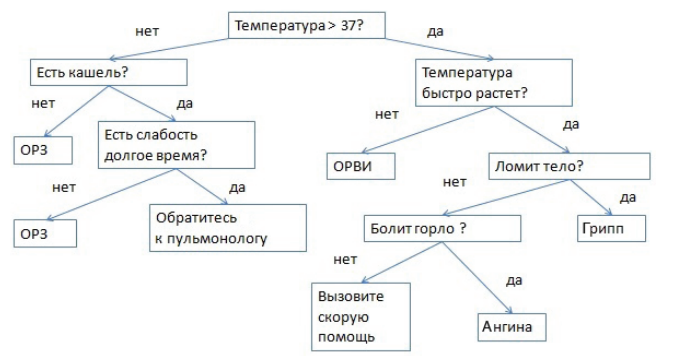
\includegraphics[scale=1]{tools/tree-ex.png}
	\caption{Пример решающего дерева}
	\label{tree}
\end{figure}

\section{Случайный лес}

В методе случайного леса (СЛ) обучают каждый алгоритм из композиции, а ответом является усредненный результат по всем 
алгоритмам, входящим в композицию.

В случае регрессии ответ а(х) находится по формуле~\ref{rand}.
\begin{equation}
	\label{rand}
	a(x) = \frac{1}{N} \sum \limits_{i=1}^{N} b_n(x)
\end{equation}
где $N$ --- количество деревьев в лесу, $b_i(x)$ --- результат i-ого алгоритма~\cite{limanovskaya}.

\section{Регрессия Гауссовского процесса}

Gaussian Process Regression (GPR) --- это гибкая непараметрическая техника регрессии. Она особенно полезна при работе с 
непрерывными данными, где связь между входными переменными и выходом не известна явно~\cite{kashtaeva}.

\chapter{Сравнение методов}

\section{Критерии сравнения}

В таблице~\ref{tbl:crits} приведены критерии для сравнения методов прогнозирования временных рядов и их описание.
\begin{table}[h]
\begin{center}
\caption{\label{tbl:crits} Критерии для сравнения методов прогнозирования временных рядов}
\begin{tabular}{| p{4cm} | p{12cm} |}
\hline
Критерий  & Описание \\
\hline
Параметры & Какие параметры, влияющие на прогноз, есть у метода \\
\hline
Дискретность & Поддерживает ли метод временные ряды, заданные дискретно \\
\hline
Непрерывность & Поддерживает ли метод временные ряды, заданные непрерывно \\
\hline
Сезонность & Поддерживает ли метод прогнозирование на данных с ярко выраженной сезонностью \\
\hline
Многомерность & Поддерживает ли метод прогнозирование многомерных данных \\
\hline
Композиция & Является ли метод композицией других методов \\
\hline
\end{tabular}
\end{center}
\end{table}

\section{Сравнение}

В таблицe~\ref{tbl:compare_res} представлены результаты сравнения методов прогнозирования временных рядов по заданным 
выше критериям.
\begin{table}[h]
	\begin{center}
	\caption{\label{tbl:compare_res} Результаты сравнения методов прогнозирования временных рядов}
	\begin{tabular}{|c|c|c|c|c|c|c|}
		\hline
		Метод & ARIMA & SARIMA & VAR & РД & СЛ & GPR \\
		\hline
		Параметры & p, d, q & p, d, q, s & p & $X_m$, j, t & $X_m$, j, t & --- \\
		\hline
		Дискретность & Да & Да & Да & Да & Да & Нет \\
		\hline
		Непрерывность & Нет & Нет & Нет & Да & Да & Да \\
		\hline
		Сезонность & Нет & Да & Да & Да & Да & Нет \\
		\hline
		Многомерность & Нет & Нет & Да & Да & Да & Нет \\
		\hline
		Композиция & Нет & Нет & Нет & Нет & Да & Нет \\
		\hline
	\end{tabular}
	\end{center}
\end{table}

\clearpage\ssr{ЗАКЛЮЧЕНИЕ}

Цель данной работы была достигнута:  исследованы методы хранения и прогнозирования временных рядов. Были решены все 
задачи:
\begin{itemize}
	\item[---] формализована задача прогнозирования временных рядов;
	\item[---] проанализированы основные методы решения задачи;
	\item[---] сформулированы критерии для сравнения методов решения задачи;
	\item[---] по сформулированным критериям проведено сравнение методов решения задачи.
\end{itemize}

\addcontentsline{toc}{chapter}{СПИСОК ИСПОЛЬЗОВАННЫХ ИСТОЧНИКОВ}
\renewcommand{\bibname}{СПИСОК ИСПОЛЬЗОВАННЫХ ИСТОЧНИКОВ}
\begin{thebibliography}{}
	\bibitem{kizbek} К.О. Кизбикенов. Прогнозирование и временные ряды. --- Город: Барнаул, 
	АлтГПУ, 2017. --- 115 с.
	\bibitem{afanas} В.Н. Афанасьев. Анализ временных рядов и прогнозирование. --- Город: Саратов, Оренбург, Ай Пи Эр 
	Медиа, 2020, 286 с.
	\bibitem{kashtaeva} С.В. Каштаева. Методы оптимизация. --- Город: Пермь, ИПЦ «Прокростъ», 2020, 84 с.
	\bibitem{itmo} А.А. Хватов, Н.О. Никитин, А.В. Калюжная. Современные методы оптимизации с примерами на Python. --- 
	Город: Санкт-Петербург, Редакционно-издательский отдел Университета ИТМО, 2023, 53 с.
	\bibitem{mayorova} Н. Л. Майорова, Д. В. Глазков. Методы оптимизации. --- Город: Ярославль, ЯрГУ, 2015, 112 с.
	\bibitem{limanovskaya} О. В. Лимановская, Т. И. Алферьева. Основы машинного обучения. --- Город: Екатеринбург,
	Издательство Уральского университета, 2020, 92 с.
	\bibitem{nosko} В.П.Носко. Эконометрика. Введение в регрессионный анализ временных рядов, --- Город: Москва, 2002, 
	254 с.
	\bibitem{box} G.E.P. Box, G.M. Jenkins и Wisconsiv Univ Madison.  <<Dept. of statistics. Time Series Analysis: Forecasting and 
	Control. Holden-Day series in time series analysis and digital processing>>, Holden-Day, 1970
	\bibitem{china} Jian Cao, Zhi Li и Jian Li. <<Financial time series forecasting model based on CEEMDAN and LSTM>>. В: Physica A: 
	Statistical Mechanics and its Applications 519 (2019), с. 127—139.
	\bibitem{martin} Martin Sundermeyer, Ralf Shluter и Hermann Ney, <<LSTM Neural Networks for Language Modeling>>, 2012
	\bibitem{deeplearning} Suman Kalyan Adari Sridhar Alla. Beginning Anomaly Detection Using Python-Based Deep Learning, 2019, 
	538 c.
\end{thebibliography}

\clearpage\ssr{ПРИЛОЖЕНИЕ А}

\begin{center}\large\textbf{Презентация к научно-исследовательской работе}\end{center}

Презентация к научно-исследовательской работе содержит 3 слайда.

\end{document}